%!TEX TS-program = xelatex
\documentclass[]{friggeri-cv}
\usepackage{afterpage}
\usepackage{hyperref}
\usepackage{color}
\usepackage{xcolor}
\usepackage{smartdiagram}
\usepackage{fontspec}
% if you want to add fontawesome package
% you need to compile the tex file with LuaLaTeX
% References:
%   http://texdoc.net/texmf-dist/doc/latex/fontawesome/fontawesome.pdf
%   https://www.ctan.org/tex-archive/fonts/fontawesome?lang=en
%\usepackage{fontawesome}
%\oddsidemargin=-1cm
\textwidth=15cm
%\marginparwidth = -3cm
\textheight=26cm

\usepackage{metalogo}
\usepackage{dtklogos}
\usepackage[utf8]{inputenc}
\usepackage{tikz}
\usetikzlibrary{mindmap,shadows}
\hypersetup{
    pdftitle={},
    pdfauthor={},
    pdfsubject={},
    pdfkeywords={},
    colorlinks=false,           % no lik border color
    allbordercolors=white       % white border color for all
}
\smartdiagramset{
    bubble center node font = \footnotesize,
    bubble node font = \footnotesize,
    % specifies the minimum size of the bubble center node
    bubble center node size = 0.5cm,
    %  specifies the minimum size of the bubbles
    bubble node size = 0.5cm,
    % specifies which is the distance among the bubble center node and the other bubbles
    distance center/other bubbles = 0.3cm,
    % sets the distance from the text to the border of the bubble center node
    distance text center bubble = 0.5cm,
    % set center bubble color
    bubble center node color = pblue,
    % define the list of colors usable in the diagram
    set color list = {lightgray, materialcyan, orange, green, materialorange, materialteal, materialamber, materialindigo, materialgreen, materiallime},
    % sets the opacity at which the bubbles are shown
    bubble fill opacity = 0.6,
    % sets the opacity at which the bubble text is shown
    bubble text opacity = 0.5,
}

\addbibresource{bibliography.bib}
\RequirePackage{xcolor}
\definecolor{pblue}{HTML}{0395DE}

\begin{document}
\header{\hspace{5.3cm}Víctor Miguel }{García Sánchez}
      {
      		\hspace{5.3cm}\begin{tabular}{l r}
		Pasante de la Maestría en Matemáticas&\color{gray}
			\normalsize
			{
			\begin{tabular}{r}
				Áreas de interés:\\ 
				\hspace{0.4cm}\scriptsize\begin{tabular}{l r r}
					\textbf{FINANZAS MATEMÁTICAS}&\hspace{0.2cm} &\textbf{MUESTREO}\\
					\textbf{CIENCIA DE DATOS}& &\textbf{MODELACIÓN}\\
				\end{tabular}
			\end{tabular}
			}
		\end{tabular}
	}

% Fake text to add separator      
\vspace{0.5cm}
\fcolorbox{white}{gray}{\parbox{\dimexpr\textwidth-2\fboxsep-2\fboxrule}{%
.....
}}

% In the aside, each new line forces a line break
\begin{aside}
  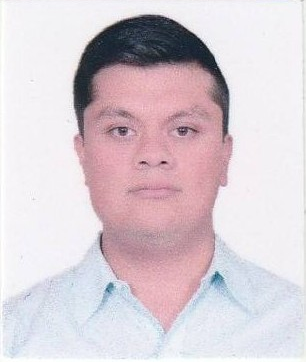
\includegraphics[scale=0.268]{img/foto2.png}
  \section{Teléfono}
    +52 5531560997\vspace{0.5cm}
  \section{Mail}
    \href{mailto:victorm.garcia@comunidad.unam.mx}{\textbf{victorm.garcia@}\\comunidad.unam.mx}\vspace{0.5cm}
    \href{mailto:victor.garcia@cimat.mx}{\textbf{victor.garcia@}\\cimat.mx}\vspace{0.5cm}
    \section{Linkedin}
    \href{linkedin.com/in/víctorm-garcia}{linkedin.com/in/víctorm-garcia}\vspace{0.5cm}
     \section{Idiomas adicionales}
    \textbf{Inglés Intermedio-Avanzado}\vspace{0.5cm}
  % use  \hspace{} or \vspace{} to change bubble size, if needed
  \section{Software}
   \smartdiagram[bubble diagram]{
       \textbf{\vspace{1mm}R},
       \textbf{\vspace{1mm}Hadoop},
       \textbf{C/C++},
        \textbf{\vspace{1mm}Python},
        \textbf{\vspace{1mm}Git},
        \textbf{\vspace{1mm}Office},
        \textbf{\vspace{-2mm}SQL}
    }\vspace{0.5cm}
  \section{Competencias y habilidades}
    \smartdiagram[bubble diagram]{
       \textbf{\vspace{2mm}Resiliencia},
	\textbf{Pensamiento}\\\textbf{crítico},
	 \textbf{Solución de}\\\textbf{problemas}\\\textbf{complejos},
	\textbf{Inteligencia}\\\textbf{emocional},
        \textbf{\vspace{1mm}Colaboración},
        \textbf{\vspace{1mm}Visualización}\\\textbf{de datos},
        \textbf{\vspace{0mm}Vinculación}\\\textbf{empresarial\vspace{-1mm}}
    }
    ~
\end{aside}
\textbf{Objetivo profesional:}
Incorporarme al área investigación económica para ampliar mis conocimientos prácticos en finanzas y estadística. Contribuir de manera positiva con el área administrativa para mejorar los procesos y resultados.
\vspace{-0.4cm}
\section{Experiencia profesional}
\begin{entrylist}
\entry
   {   \begin{tabular}{r}
    		01/20\\
     		\hspace{0.87cm}
\includegraphics[scale=0.15]{img/hdi.png}
	\end{tabular}
    }
    {\vspace{-0.91cm}}
    { }
    {Participación en el proyecto \textsl{Estimation of Future Property Insurance Cancellations} en el marco del \textbf{13o. Taller de Solución de Problemas Industriales} llevado a cabo en el Centro de Investigación en Matemáticas.}
\entry
    {   \begin{tabular}{r}
    		01/19- a la fecha  \\
     		
\includegraphics[scale=0.09]{img/unitips.jpg}
	\end{tabular}
    }
    {\vspace{-1.05cm}}
    { }
    {Tutor del área de matemáticas del curso Unitips de ingreso a la universidad, brindando asesorías a aspirantes a estudiar en la UNAM, IPN, UAM, entre otros.}
\entry
   {   \begin{tabular}{r}
    		08/18-11/18\\
     		
\includegraphics[scale=0.15]{img/RAI.jpg}
	\end{tabular}
    }
    {\vspace{-0.95cm}}
    { }
    {Participación en el proyecto de investigación \textsl{Modelos espaciales predictivos para la obesidad, el síndrome metabólico, la diabetes tipo 2 y enfermedades cardiovasculares en México}.}
  \entry
    {\begin{tabular}{r}
    		06/18-07/18\\
     		
\includegraphics[scale=0.203]{img/20verano.jpeg}
	\end{tabular}\hspace{0.4cm}
    }
    {\vspace{-0.98cm}}
    { }
    {Investigación en el proyecto \textsl{Sobre la luminosidad emitida por máseres de agua en función de otras variables}, sobre estadística y astroquímica, asesorado por investigadores del Departamento de Astronomía de la Universidad de Guanajuato (UG).}% Dicho proyecto destacó y será incluido en la Memoria del 20° Verano de la Ciencia Región Centro.\\}
  \entry
    {   \begin{tabular}{r}
    		09/15 - 06/18\\
     		\hspace{0.9cm}
\includegraphics[scale=0.5]{img/UGTO.png}
	\end{tabular}
    }
    {\vspace{-1.51cm}}
    { }
    {Ayudante de cátedra, encargado de realizar la evaluación de tareas, aplicación de exámenes y responsable de sesiones de estudio en distintos cursos de las licenciaturas en matemáticas, computación y química, además de ingenierías en minas y química. Se logró una mejora en las evaluaciones de los alumnos de todos los grupos.}
\end{entrylist}
\section{Educación}
\begin{entrylist}
  \entry
     {   \begin{tabular}{l}
    		\hspace{0.8cm}2018-2020\\
     		\hspace{0.9cm}
\includegraphics[scale=0.4]{img/iimas.png}
	\end{tabular}
    }
    {\vspace{-1.46cm}}
    { }
    {\textbf{Pasante de la Maestría en Ciencias Matemáticas} con orientación a Finanzas matemáticas. Inscrito al Instituto de Investigaciones en Matemáticas Aplicadas y en Sistemas de la Universidad Nacional Autónoma de México, con la tesis \textsl{La volatilidad de un activo como movimiento Browniano fraccionario}.}
    \entry
    {   \begin{tabular}{l}
    		\hspace{0.8cm}2013-2018\\
     		\hspace{0.9cm}
\includegraphics[scale=0.5]{img/UGTO.png}
	\end{tabular}
    }
    {\vspace{-1.49cm}}
    { }
    {\textbf{Licenciado en Matemáticas} por la Universidad de Guanajuato, con la tesis \textsl{Estimador por calibración: Problemas en su implementación y propuestas de soluciones}.}
    \entry
    {   \begin{tabular}{l}
    		\hspace{0.8cm}2010-2013\\
     		\hspace{0.9cm}
\includegraphics[scale=0.21]{img/cbtis.png}
	\end{tabular}
    }
    {\vspace{-1.39cm}}
    { }
    {\textbf{Técnico bachiller en Mecatrónica} por el Centro de Bachillerato Tecnológico industrial y de servicios 59 ``Miguel Hidalgo y Costilla''.}
    \end{entrylist}
    \newpage
\begin{aside}
~
~
~
	\section{Manejo de Sistemas Operativos}
    \textbf{GNU/Linux}
\includegraphics[scale=0.40]{img/5stars.png}
    \textbf{Windows}
\includegraphics[scale=0.40]{img/4stars.png}
    \textbf{Mac OS}
\includegraphics[scale=0.40]{img/4stars.png}
	\section{Certificados}
	~
     	
\includegraphics[scale=0.04]{img/Microsoft.jpg}
	\textbf{Competencias tecnológicas para la productividad}, 2011.
	
\includegraphics[scale=0.2]{img/ucdavis.jpg}
	\textbf{SQL for Data Science}, 2020.
%	
\includegraphics[scale=0.2]{img/ucdavis.jpg}
%	\textbf{SQL for Data Science}, 2020.
	\section{Cursos}
	~
	
\includegraphics[scale=0.08]{img/santander.png}
\includegraphics[scale=0.08]{img/ie.png}
	\textbf{DATA SCIENCE, MACHINE LEARNING AND AI FOR BUSINESS}, 2020.
	
\includegraphics[scale=0.15]{img/cimat.png}
	\textbf{Data Science Fin-ML/IVADO Workshop Montreal-Guanajuato}, 2020.
	
\includegraphics[scale=0.025]{img/UDLAP.jpg}
	\textbf{I Taller Inter-Institucional de Ciencia de Datos e Inteligencia Artificial}, 2019.
	
\includegraphics[scale=0.04]{img/ciencias.png}
	\textbf{Quinto Congreso de Actuaría}, 2019.
	
\includegraphics[scale=0.04]{img/inegi.jpg}
	\textbf{Seminario internacional sobre edición de datos, imputación y no respuesta}, 2017.
	
\includegraphics[scale=0.25]{img/hollington.png}
	\textbf{Life Styles}, Curso de Inglés, 2007-2009.
\end{aside}
\section{Formación de capital humano}
\begin{entrylist}
    \entry
     {   \begin{tabular}{l}
    		\hspace{0.9cm}2019\\
     		
\includegraphics[scale=0.15]{img/mexicanas.png}
	\end{tabular}
    }
    {\vspace{-0.99cm}}
    { }
    {\textbf{Colaborador en Mexicanas del Futuro: Trazando Conciencias, Pensando en TI}, efectuando actividades de apoyo en la organización de la feria de talleres orientada a motivar la vocación científica en las jóvenes de preparatoria, llevado a cabo en las instalaciones del IIMAS.}
 \entry
    {   \begin{tabular}{l}
    		\hspace{0.8cm}2016\\
     		\hspace{0.4cm}
\includegraphics[scale=0.5]{img/UGTO.png}
	\end{tabular}
    }
    {\vspace{-1.49cm}}
    { }
    {\textbf{Principal ponente y organizador} del seminario semanal de Artificios de Integración.}
\entry
     {   \begin{tabular}{l}
    		\hspace{0.9cm}2015\\
     		\hspace{0.5cm}
\includegraphics[scale=0.2]{img/cimat.png}
	\end{tabular}
    }
    {\vspace{-1.4cm}}
    { }
    {\textbf{Ponente} del Curso para entrenadores de la Olimpiada de Matemáticas, dirigido a profesores de preparatoria con el tema “Teoría de números”.}
    \entry
     {   \begin{tabular}{l}
    		\hspace{0.3cm}2013-2015\\
     		\hspace{0.5cm}
\includegraphics[scale=0.23]{img/ommgto.jpg}
	\end{tabular}
    }
    {\vspace{-1.27cm}}
    { }
    {\textbf{Entrenador de la preselección del estado de Guanajuato}, además del apoyo en la elaboración, aplicación y evaluación de los exámenes selectivos de cada etapa.}
\end{entrylist}
\vspace{-0.5cm}
\section{Publicaciones}
García Sánchez, Víctor Miguel y Trinidad Hernández, Miguel Ángel\\
\textbf{Sobre la luminosidad emitida por máseres de agua en función de otras variables}\\
\emph{20° Verano de la Ciencia Región Centro, Vol 4. Núm. 7.}
\section{Reconocimientos y distinciones}
\begin{entrylist}
  \entry
    {\hspace{0.9cm}2019}
    {Mención honorífica en la Sesión de Carteles de la XVII Escuela de\\Probabilidad y Estadística}
    {Concurso de carteles}
    {Por la presentación del cartel \emph{“INLA como alternativa a MCMC y su uso en un modelo predictivo espacial”}.}
    \entry
    {\hspace{0.9cm}2013}
    {Primer lugar nacional de la primera etapa}
    {Festival Académico 2013}
    {Galardón obtenido en el área de matemáticas del concurso organizado por la Dirección General de Educación Tecnológica Industrial.}
    \entry
    {\hspace{0.9cm}2012}
    {Medalla de bronce}
    {26 Olimpiada Mexicana de Matemáticas}
    {Obtenida por puntaje en la participación en la etapa nacional de la 26a OMM celebrada en la ciudad de Guanajuato, Gto., siendo invitado a realizar los estudios de la Licenciatura en Matemáticas en la misma ciudad por personal del Centro de Investigación  en Matemáticas.}
    \entry
    {\hspace{0.9cm}2011}
    {Mención honorífica}
    {25 Olimpiada Mexicana de Matemáticas}
    {Obtenida por puntaje en la participación en la etapa nacional de la 25a OMM celebrada en la ciudad de San Luis Potosí, SLP.}
    \entry
    {\hspace{0.9cm}2010}
    {Primer lugar del estado de Hidalgo y participación en la etapa nacional}
    {ExpoCiencias}
    {Participando con proyecto de investigación sobre el número $\pi$ (pi).}
    \entry
    {\hspace{0.9cm}2008}
    {Seleccionado nacional}
    {12th Po Leung Kuk Primary Mathematics World Contest}
    {Participación en el concurso internacional Po Leung Kuk celebrado en Hong Kong.}
    \entry
    {\hspace{0.9cm}2006}
    {Primer lugar estatal en matemáticas}
    {Examen ENLACE}
    {Mejor puntaje en el examen ENLACE siendo invitado a la ceremonia de premiación en la residencia oficial de Los Pinos.}
\end{entrylist}

%\section{Información adicional}
%\emph{ }
%\\

\end{document}%\section{Publications}%Author, Author, Author\\